\documentclass[aspectratio=169,11pt]{beamer}

\usepackage[utf8]{inputenc}
\usepackage[T1]{fontenc}
\usepackage{tikz}
\usetikzlibrary{arrows.meta,positioning,shapes.geometric}

% ---------- Theme ----------
\usetheme{Madrid}
% Dark palette
\definecolor{bgdark}{RGB}{16,22,36}      % slide background
\definecolor{bgpanel}{RGB}{28,38,58}     % header/footer + block bodies
\definecolor{fgtext}{RGB}{226,232,243}   % main text
\definecolor{ltublue}{RGB}{111,168,255}  % accent (light blue, readable on dark)
\definecolor{alertcol}{RGB}{255,171,92}  % alert accent (orange)

\setbeamercolor{normal text}{fg=fgtext,bg=bgdark}
\setbeamercolor{background canvas}{bg=bgdark}
\setbeamercolor{structure}{fg=ltublue}
\setbeamercolor{palette primary}{bg=bgpanel,fg=fgtext}
\setbeamercolor{palette secondary}{bg=bgpanel!80!black,fg=fgtext}
\setbeamercolor{palette tertiary}{bg=bgdark!60!black,fg=fgtext}
\setbeamercolor{frametitle}{bg=bgpanel,fg=ltublue}
\setbeamercolor{title}{bg=bgpanel,fg=ltublue}
\setbeamercolor{titlelike}{fg=ltublue}
\setbeamercolor{block title}{bg=ltublue!35!bgpanel,fg=fgtext}
\setbeamercolor{block body}{bg=bgpanel,fg=fgtext}
\setbeamercolor{block title alerted}{bg=alertcol!40!bgpanel,fg=fgtext}
\setbeamercolor{block body alerted}{bg=bgpanel,fg=fgtext}
\setbeamercolor{alerted text}{fg=alertcol}
\setbeamercolor{item}{fg=ltublue}
\setbeamercolor{footnote}{fg=fgtext!70!bgdark}
\setbeamercolor{footnote mark}{fg=ltublue}
\setbeamercolor{section in toc}{fg=fgtext}
\setbeamercolor{description item}{fg=ltublue}
\setbeamercolor{enumerate item}{fg=ltublue}
\setbeamercolor{caption name}{fg=ltublue}
\setbeamercolor{item projected}{bg=ltublue,fg=bgdark}  % numbered bullets: dark digit on light-blue disc
\setbeamercolor{subitem projected}{bg=ltublue,fg=bgdark}
\setbeamertemplate{navigation symbols}{}
\setbeamertemplate{itemize items}[circle]
\setbeamertemplate{enumerate items}[circle]   % flat disc, no glossy highlight
\setbeamerfont{footnote}{size=\tiny}

% ---------- Title info ----------
\title[Adaptive Human--AI Task Allocation]{Adaptive Human--AI Task Allocation}
\subtitle{Start Seminar}
\author{Yaser Kaddoura}
\institute[LTU]{%
  Lule\r{a} University of Technology\\[2pt]
  {\small Principal supervisor: Prof.\ Ahmed Elragel\\
  Assistant supervisor: Senior Lecturer J\"orgen Nilsson}}
\date{November 4, 2026}
% \titlegraphic{
\includegraphics[height=1.2cm]{ltu_logo.png}}

\pdfstringdefDisableCommands{\def\translate#1{#1}} % silences hyperref warning caused by \appendix
\begin{document}

% ======================================================
\begin{frame}
  \titlepage
\end{frame}

\begin{frame}{Outline}
  \tableofcontents
\end{frame}

% ======================================================
\section{Problem and Solution}

\begin{frame}{Context}
  \begin{itemize}
    \item AI is increasingly embedded in work and decision-making
    \begin{itemize}
      \item Generates content, predicts, recommends, acts with varying autonomy
      \item Professional work, public services, consumer applications
    \end{itemize}
    \item Capable, but not uniformly reliable, especially in sensitive tasks
    \item Hence the interest in human--AI collaboration: \textbf{hybrid intelligence} [3]
  \end{itemize}
\end{frame}

\begin{frame}{The shift in focus}
  \begin{columns}[T]
    \begin{column}{0.45\textwidth}
      \begin{block}{From}
        Can AI do this task in isolation?
      \end{block}
    \end{column}
    \begin{column}{0.45\textwidth}
      \begin{block}{To}
        How should humans and AI be organised to do it well?
      \end{block}
    \end{column}
  \end{columns}
  \vspace{1em}
  \textbf{Task allocation} = how the following are distributed between human and AI:
  \begin{itemize}
    \item Work
    \item Information
    \item Decision authority
    \item Accountability
  \end{itemize}
\end{frame}

\begin{frame}{Why static allocation fails}
  \begin{itemize}
    \item Examples: always automate, always require human review, same workflow for every task
    \item Human--AI teams do not necessarily outperform their best member [2]
    \item Consequences
    \begin{itemize}
      \item Over- or under-reliance on AI
      \item Wasted human effort and expertise
      \item Human review becomes nominal rather than meaningful [7]
      \item Accountability falls on operators without real control [6]
    \end{itemize}
  \end{itemize}
\end{frame}

\begin{frame}{Gap and proposed solution}
  \begin{itemize}
    \item \textbf{Gap}: knowledge is fragmented across conceptual, behavioural,
      organisational, and technical perspectives
    \item Not yet integrated into adaptive approaches for practical settings
  \end{itemize}
  \vspace{1em}
  \begin{alertblock}{Proposed solution}
    An adaptive allocation framework that decides, per task, whether it goes to
    an \textbf{AI}, a \textbf{human}, or a \textbf{human--AI arrangement}
  \end{alertblock}
\end{frame}

% ======================================================
\section{Research Questions}

\begin{frame}{Research questions}
  \begin{block}{Main RQ}
    How should a human--AI system decide whether a task should be handled by an AI,
    a human, or a combination of both?
  \end{block}
  \begin{description}
    \item[RQ1 (design)] How can an adaptive human--AI task-allocation framework be
      designed, drawing on task-, AI-, human-, and interaction-related factors?
    \item[RQ2 (evaluation)] How does the framework perform compared with relevant
      fixed or non-adaptive allocation approaches under defined evaluation conditions?
  \end{description}
\end{frame}

% ======================================================
\section{Literature Review}

\begin{frame}{Literature review: four perspectives}
  \begin{itemize}
    \item Conceptual, behavioural, organisational, and technical perspectives
    \item Grouped here into three streams:
    \begin{enumerate}
      \item Human factors and appropriate reliance
      \item Allocation structures and collaboration patterns
      \item Technical approaches to delegation
    \end{enumerate}
  \end{itemize}
\end{frame}

\begin{frame}{Human factors and appropriate reliance}
  \begin{itemize}
    \item Accuracy alone does not determine team performance; mental models matter [4]
    \item Limited metaknowledge hampers delegation [9]
    \begin{itemize}
      \item AI-to-human delegation improved performance
      \item Human-to-AI delegation did not
    \end{itemize}
  \end{itemize}
\end{frame}

\begin{frame}{Allocation structures and complementarity}
  \begin{itemize}
    \item Full delegation, sequential, or aggregated decision making; appropriateness is
      context-contingent [1]
    \item Taxonomy of interaction patterns in AI-assisted decisions [10]
    \item Between-task vs.\ within-task complementarity [11]
  \end{itemize}
\end{frame}

\begin{frame}{Technical approaches and the gap}
  \begin{itemize}
    \item Learning to defer: a model either predicts or defers to a human expert [8, 12]
    \item Depends on how humans, tasks, and feedback are represented
  \end{itemize}
  \vspace{0.8em}
  \begin{alertblock}{Synthesis}
    Frameworks and taxonomies describe the options, but not how to \emph{select}
    or \emph{adapt} among them
    \begin{itemize}
      \item[$\Rightarrow$] Research opportunity
    \end{itemize}
  \end{alertblock}
\end{frame}

% ======================================================
\section{Methodology}

\begin{frame}{Design Science Research Methodology (DSRM)}
  \begin{itemize}
    \item Why DSRM: a practical design problem; an artifact to build and evaluate
    \item Peffers et al.\ (2007) [13]
    \item Iterative, not strictly sequential
  \end{itemize}
  \vspace{0.6em}
  \begin{center}
  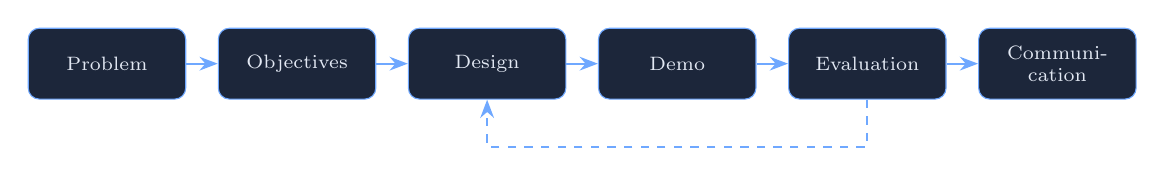
\begin{tikzpicture}[
      node distance=4mm,
      dsrmstep/.style={draw=ltublue,fill=bgpanel,text=fgtext,rounded corners,
                   minimum height=9mm,minimum width=20mm,align=center,font=\scriptsize},
      arr/.style={-{Stealth},thick,ltublue}]
    \node[dsrmstep] (a) {Problem};
    \node[dsrmstep,right=of a] (b) {Objectives};
    \node[dsrmstep,right=of b] (c) {Design};
    \node[dsrmstep,right=of c] (d) {Demo};
    \node[dsrmstep,right=of d] (e) {Evaluation};
    \node[dsrmstep,right=of e] (f) {Communi-\\cation};
    \foreach \x/\y in {a/b,b/c,c/d,d/e,e/f} \draw[arr] (\x) -- (\y);
    \draw[arr,dashed] (e.south) -- ++(0,-6mm) -| (c.south);
  \end{tikzpicture}
  \end{center}
\end{frame}

\begin{frame}{The artifact}
  \begin{itemize}
    \item A framework for adaptive task allocation in decision-making
    \item Form depends on the selected use case
    \begin{itemize}
      \item Model, method, decision procedure, or software instantiation
    \end{itemize}
    \item Recommends or determines: \textbf{AI}, \textbf{human}, or \textbf{human--AI}
  \end{itemize}
\end{frame}

\begin{frame}{Theoretical and practical foundations}
  \begin{columns}[T]
    \begin{column}{0.55\textwidth}
      \textbf{Theory}
      \begin{itemize}
        \item Types and levels of automation [14]
        \item Automation complacency and bias [15]
        \item Hybrid intelligence and organisational decision structures [3, 1]
      \end{itemize}
    \end{column}
    \begin{column}{0.4\textwidth}
      \textbf{Practice}
      \begin{itemize}
        \item Selected use case
        \item Workflows, records, observations, outcomes
      \end{itemize}
    \end{column}
  \end{columns}
  \vspace{0.8em}
  Systematic literature review as the knowledge base:
  conceptualisations, considerations, design alternatives, evaluation approaches
\end{frame}

\begin{frame}{Research process}
  \begin{enumerate}
    \item Systematic literature review
    \item Problem formulation in a selected use case
    \item Define solution objectives
    \item Design and demonstrate the artifact
    \item Evaluate
    \begin{itemize}
      \item Formative: feeds the next iteration, contributes to \textbf{RQ1}
      \item Comparative vs.\ fixed / non-adaptive approaches: answers \textbf{RQ2}
    \end{itemize}
  \end{enumerate}
  \vspace{0.5em}
  \textbf{Expected contributions:} (1) the adaptive framework; (2) comparative evidence of its performance
\end{frame}

% ======================================================
\section{Closing}

\begin{frame}{Summary}
  \begin{itemize}
    \item \textbf{Problem}: static human--AI allocation is inadequate; knowledge is fragmented
    \item \textbf{Approach}: DSRM, with an adaptive allocation framework as the artifact
    \item \textbf{Evaluation}: comparison against fixed / non-adaptive allocation
  \end{itemize}
\end{frame}

\begin{frame}[plain]
  \centering
  \vfill
  {\Huge\bfseries\color{ltublue} Open Discussion}
  \vfill
\end{frame}

% ======================================================
\appendix
\begin{frame}[allowframebreaks]{References}
  \tiny
  \begin{thebibliography}{99}
    \bibitem{1} Shrestha, Ben-Menahem, von Krogh. Organizational Decision-Making Structures in the Age of AI. \emph{California Management Review} 61(4), 2019.
    \bibitem{2} Hemmer et al. Complementarity in Human-AI Collaboration. \emph{EJIS} 34(6), 2025.
    \bibitem{3} Dellermann et al. Hybrid Intelligence. \emph{BISE} 61(5), 2019.
    \bibitem{4} Bansal et al. Beyond Accuracy: The Role of Mental Models in Human-AI Team Performance. \emph{HCOMP} 7, 2019.
    \bibitem{5} Bansal et al. Is the Most Accurate AI the Best Teammate? \emph{AAAI} 35(13), 2021.
    \bibitem{6} Elish. Moral Crumple Zones. \emph{Engaging Science, Technology, and Society} 5, 2019.
    \bibitem{7} Van Den Bosch et al. Measuring Meaningful Human Control in Human--AI Teaming. \emph{AI and Ethics} 5(3), 2025.
    \bibitem{8} Mozannar, Sontag. Consistent Estimators for Learning to Defer to an Expert. \emph{ICML}, PMLR 119, 2020.
    \bibitem{9} F\"ugener et al. Cognitive Challenges in Human--AI Collaboration. \emph{Information Systems Research} 33(2), 2022.
    \bibitem{10} Gomez et al. Human-AI Collaboration Is Not Very Collaborative yet. \emph{Frontiers in Computer Science} 6, 2025.
    \bibitem{11} F\"ugener, Walzner, Gupta. Roles of AI in Collaboration with Humans. \emph{Management Science} 72(1), 2026.
    \bibitem{12} Strong et al. Learning to Defer: A Survey. 2025.
    \bibitem{13} Peffers et al. A Design Science Research Methodology for Information Systems Research. \emph{JMIS} 24(3), 2007.
    \bibitem{14} Parasuraman, Sheridan, Wickens. A Model for Types and Levels of Human Interaction with Automation. \emph{IEEE Trans.\ SMC-A} 30(3), 2000.
    \bibitem{15} Parasuraman, Manzey. Complacency and Bias in Human Use of Automation. \emph{Human Factors} 52(3), 2010.
  \end{thebibliography}
\end{frame}

\end{document}
